\mode*

\section{Klasser och objekt}

Objekt är instanser av klasser.
Klasser är ritningarna, specifikationerna.

\begin{frame}[fragile]
  \begin{block}{Klass}
    \begin{itemize}
      \item En klass är en ritning eller specifikation för ett objekt.
    \end{itemize}
  \end{block}

  \begin{minted}{python}
    class Class:
      def __init__(self):
        self.__attribute = something

      def method(self):
        return self.__attribute
  \end{minted}
\end{frame}

\begin{frame}[fragile]
  \begin{block}{Objekt}
    \begin{itemize}
      \item Objekt (plural) är instanser av en klass.
    \end{itemize}
  \end{block}

  \begin{minted}{python}
    objekt1 = Class()
    objekt2 = Class()
  \end{minted}
\end{frame}


\subsection{Metoder och attribut}

\begin{frame}[fragile]
  \begin{block}{Attribut}
    \begin{itemize}
      \item Är data som tillhör objektet.
      \item Vanligtvis initierade i \mintinline{python}{__init__}.
    \end{itemize}
  \end{block}

  \begin{minted}{python}
    class Class:
      def __init__(self, attr):
        self.__attr = attr
  \end{minted}
\end{frame}

\begin{frame}[fragile]
  \begin{block}{Metoder}
    \begin{itemize}
      \item Metoder är funktioner som tillhör objektet.
      \item Dessa används för att interagera med objektet.
    \end{itemize}
  \end{block}

  \begin{minted}{python}
    class Class:
      def method(self):
        # do something object related
  \end{minted}
\end{frame}

\begin{frame}[fragile]
  person.py \hrulefill
  \inputminted[linenos,lastline=8]{python}{examples/person.py}
\end{frame}

\begin{frame}[fragile]
  person.py \hrulefill
  \inputminted[linenos,firstline=3,lastline=4]{python}{examples/person.py}
  \dots
  \inputminted[autogobble=false,linenos,firstline=10,lastline=16]{python}{examples/person.py}
\end{frame}

\begin{frame}[fragile]
  person.py \hrulefill
  \inputminted[linenos,firstline=3,lastline=5]{python}{examples/person.py}
  \dots
  \inputminted[linenos,firstline=35,lastline=39]{python}{examples/person.py}
\end{frame}


\section{Arv}

\begin{frame}[fragile]
  \begin{block}{Arv}
    \begin{itemize}
      \item En klass kan ärva en annan klass.
      \item Den kan då förbättra saker.
    \end{itemize}
  \end{block}

  \begin{minted}{python}
    class Child(Class):
      def method(self):
        """ Better method """
        return super().method()**2
  \end{minted}
\end{frame}

\begin{frame}[fragile]
  person\textunderscore nick.py \hrulefill
  \inputminted[linenos,lastline=17]{python}{examples/person_nick.py}
\end{frame}

\begin{frame}[fragile]
  \begin{remark}
    \begin{itemize}
      \item Kan även byta ut funktionalitet.
    \end{itemize}
  \end{remark}
  person\textunderscore nick.py \hrulefill
  \inputminted[linenos,firstline=19,lastline=27]{python}{examples/person_nick.py}
\end{frame}

\begin{frame}[fragile]
  person\textunderscore nick.py \hrulefill
  \inputminted[linenos,firstline=30]{python}{examples/person_nick.py}
\end{frame}


\section{Specialmetoder}

\begin{frame}[fragile]
  person\textunderscore str.py \hrulefill
  \inputminted[linenos,lastline=8]{python}{examples/person_str.py}
\end{frame}

\begin{frame}[fragile]
  person\textunderscore str.py \hrulefill
  \inputminted[linenos,firstline=11]{python}{examples/person_str.py}
\end{frame}

\begin{frame}
  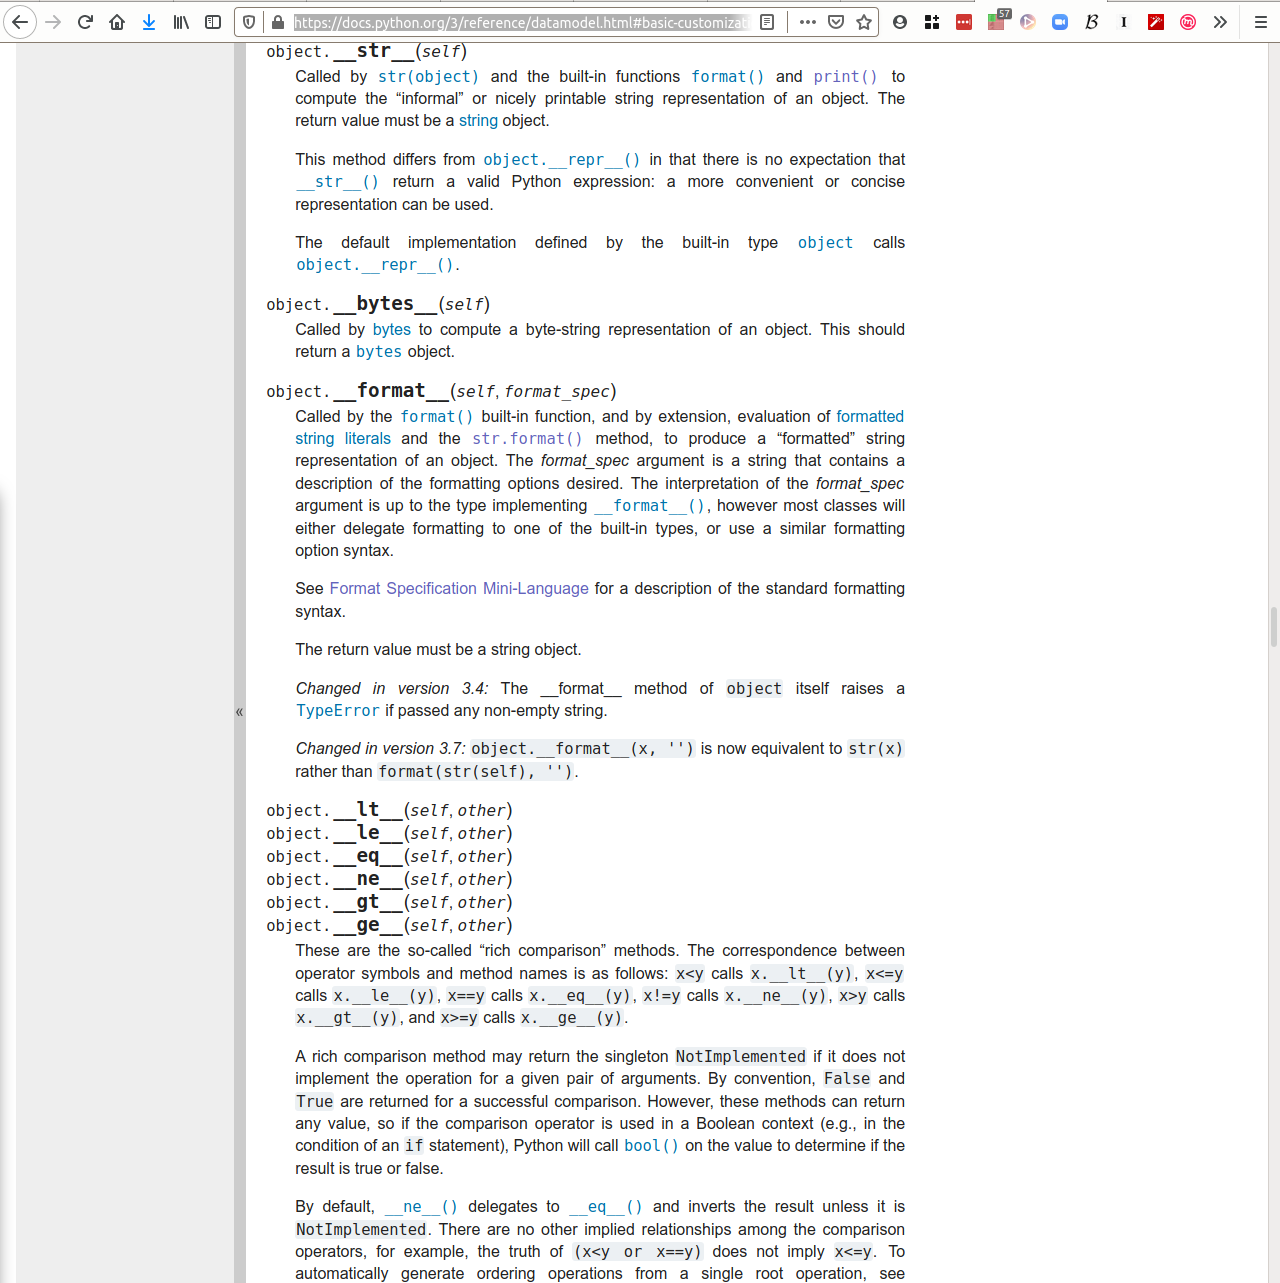
\includegraphics[width=\columnwidth]{figs/docs-special-methods.png}
\end{frame}
